\documentclass{article}
%\usepackage[screen]{geometry}
\usepackage{alltt,fancyvrb,framed,xcolor,amsmath}
\usepackage[utf8]{inputenc}
\usepackage{listings}
\usepackage{graphicx}
\usepackage{epstopdf}
\usepackage{marginnote}
\usepackage[screen, right=3.5in, marginparwidth=3in]{geometry}
\colorlet{shadecolor}{white}
\lstdefinelanguage
[x64]{Assembler}
[x86masm]{Assembler}
{
  otherkeywords={
	  movq,movl,movw,movb,
	  pushq, popq,
	  addq,addl,addw,addb,
	  subq,subl,subw,subb,
	  syscall,
	  leaq,leal,leaw,leab, 
	  xorq,xorl,xorw,xorb,
	  callq,
	  testq,testl,testw,testb,
	  cmpq,cmpl,cmpw,cmpb,
	  andq,andl,andw,andb,
	  %orq,orl,orw,orb,
	  negq,negl,negw,negb,
	  incq,incl,incw,incb,
	  decq,decl,decw,decb,
	  \%rax,\%eax,\%ax,\%al,
	  \%rdx,\%edx,\%dx,\%dl,
	  \%rcx,\%ecx,\%cx,\%cl,
	  \%rbx,\%ebx,\%bx,\%bl,
	  \%rsi,\%esi,\%si,\%sil,
	  \%rdi,\%edi,\%di,\%dil,
	  \%rsp,
	  \%rbp,
	  \%r8,\%r8d,\%r8w,\%r8b,
	  \%r9,\%r9d,\%r9w,\%r9b,
	  \%r10,\%r10d,\%r10w,\%r10b,
	  \%r11,\%r11d,\%r11w,\%r11b,
	  \%r12,\%r12d,\%r12w,\%r12b,
	  \%r13,\%r13d,\%r13w,\%r13b,
	  \%r14,\%r14d,\%r14w,\%r14b,
	  \%r15,\%r15d,\%r15w,\%r15b
	  }
}
\lstset{
 belowcaptionskip=1\baselineskip,
 xleftmargin=\parindent,
 breaklines=true, %% Wrap long lines
 language=[x64]Assembler,
 escapeinside={/*}{*/},
 escapebegin=\begin{shaded}\obeyspaces\obeylines,
 escapeend=\end{shaded},
 showstringspaces=false,
 basicstyle=\small\ttfamily,
 commentstyle=\itshape\color{gray},
 stringstyle=\color{black},
 keywordstyle=\bfseries\color{green},
 identifierstyle=\color{blue},
 %numbers=left,
}
\begin{document}

\section*{Specification}
\lstinputlisting{Specification.txt}

\newpage\section*{HTML Page}
\lstinputlisting{Page.html}

\newpage\section*{Start}
\lstinputlisting{Start.s}

\newpage\section*{Main}
\lstinputlisting{Main.s}

\newpage\section*{GetENV}
\lstinputlisting{GetENV.s}

\newpage\section*{Query}
\lstinputlisting{Query.s}

\newpage\section*{HTMLHeader}
\lstinputlisting{HTMLHeader.s}

\newpage\section*{PrintHTMLImage}
\lstinputlisting{PrintHTMLImage.s}

\newpage\section*{Process}
\lstinputlisting{Process.s}

\newpage\section*{Plot}
\lstinputlisting{Plot.s}

\newpage\section*{Output}
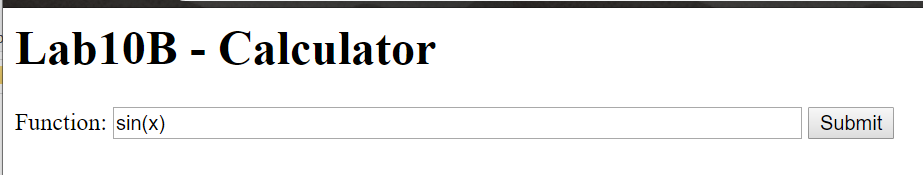
\includegraphics[width=\textwidth]{Output_1.png}
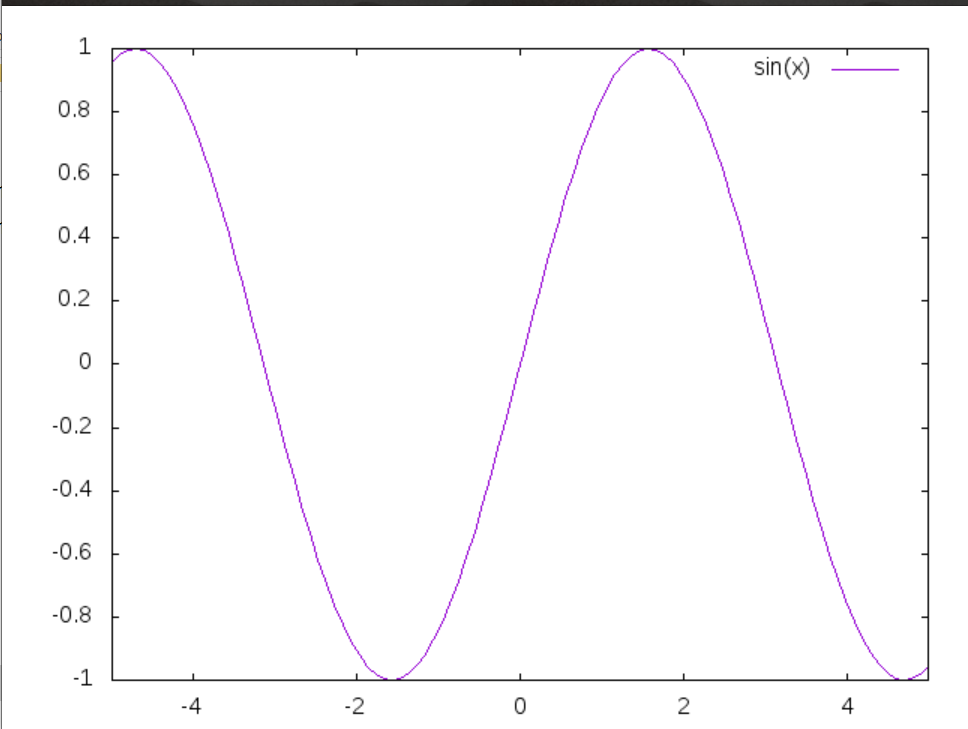
\includegraphics[width=\textwidth]{Output_1_2.png}
\newpage
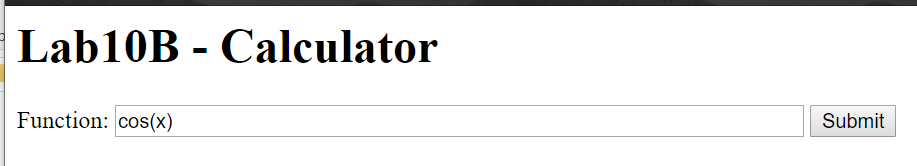
\includegraphics[width=\textwidth]{Output_2.png}
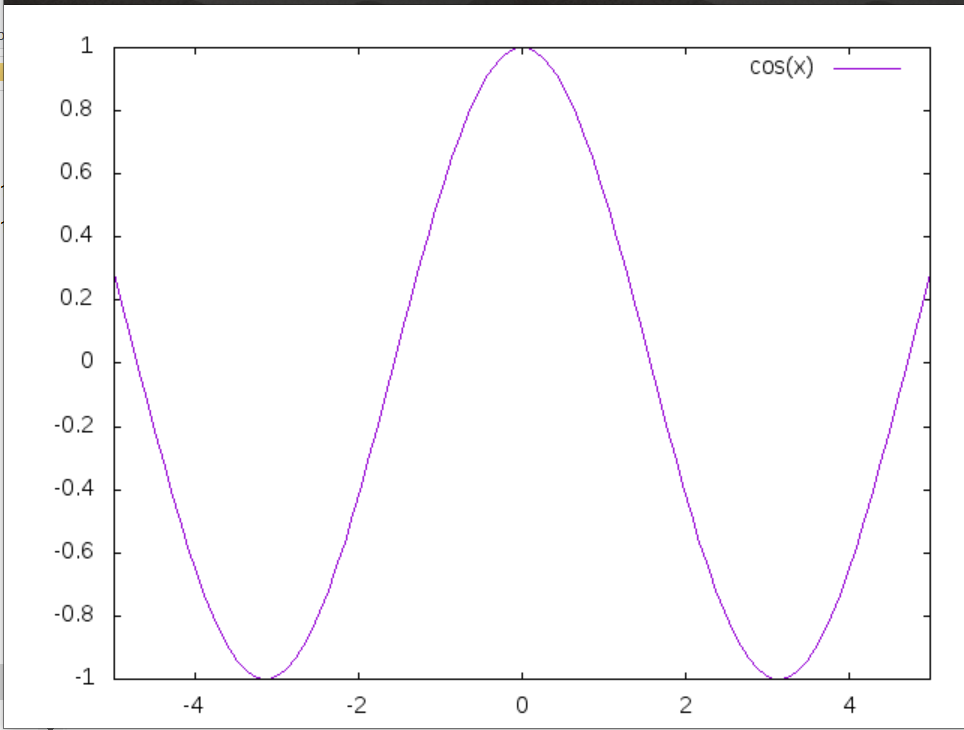
\includegraphics[width=\textwidth]{Output_2_2.png}

\marginnote{}

\end{document}
